\documentclass{article}
\usepackage{graphicx}
\usepackage{xcolor}
\usepackage{multirow}

\begin{document}

\section{Table Example}
\begin{center}
\begin{tabular}{|c|c|c|}
\hline
Name & Subject & Marks \\
\hline
Asha & Maths & 90 \\
Ravi & Science & 85 \\
\hline
\end{tabular}
\end{center}

\section{Colour Example}
\textcolor{blue}{This text is blue.}

\definecolor{myblue}{RGB}{10,60,200}
\textcolor{myblue}{This text uses a custom colour.}

\section{Figure Example}

\begin{figure}[h]
     \centering
     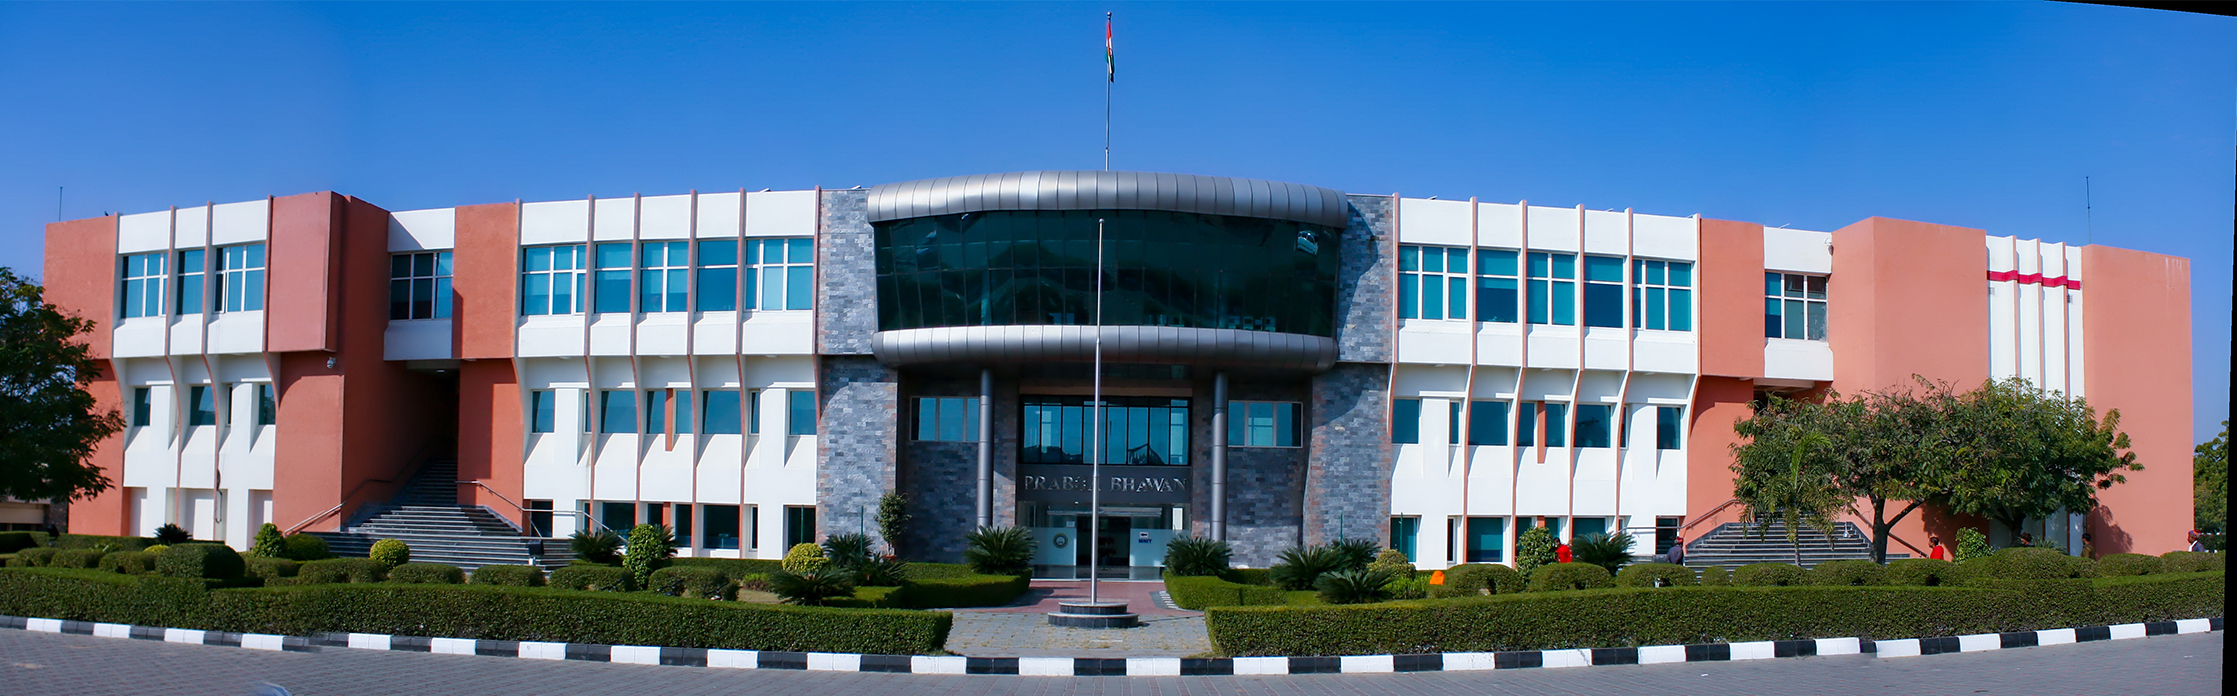
\includegraphics[width=0.5\textwidth]{pb_mnit.jpg}
     \caption{Sample image}
\end{figure}

\end{document}